\documentclass{amsart}
\usepackage{amsmath}
\usepackage{amssymb}
\usepackage{tikz}
\usepackage[utf8]{inputenc}
\usepackage{pgfplots}
\usepackage{color}
\usetikzlibrary{decorations.markings}
\usetikzlibrary{arrows.meta}

\begin{document}

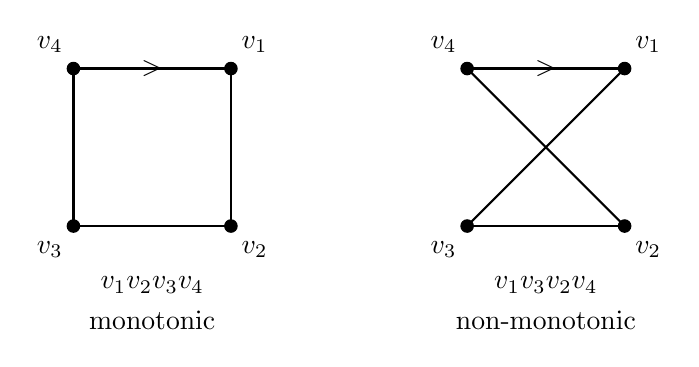
\begin{tikzpicture} \draw[fill=black] (1,1) circle
(2.25pt); \draw[fill=black] (-1,1) circle (2.25pt); \draw[fill=black] (1,-1)
circle (2.25pt); \draw[fill=black] (-1,-1) circle (2.25pt);
    
	\draw[thick] (1,1) -- (1,-1); \draw[thick] (1,-1) -- (-1,-1); \draw[thick,]
	(-1,-1) -- (-1,1); \draw[thick] (-1,1) -- (1,1);
    
	\node[] at (0,1) ($>$){$>$};
    
	\node[] at (1.3,1.3) (1){$v_1$};
	\node[] at (1.3,-1.3) (2){$v_2$};
	\node[] at (-1.3,-1.3) (3){$v_3$};
	\node[] at (-1.3,1.3) (4){$v_4$};
    
	\node[] at (0,-1.75) (1234){$v_1v_2v_3v_4$};
	\node[] at (0,-2.2) {monotonic};
	\draw[fill=black] (6,1) circle (2.25pt); \draw[fill=black] (4,1) circle
	(2.25pt); \draw[fill=black] (6,-1) circle (2.25pt); \draw[fill=black]
	(4,-1) circle (2.25pt);
    
	\draw[thick] (6,1) -- (4,-1); \draw[thick] (6,-1) -- (4,1); \draw[thick,]
	(4,-1) -- (6,-1); \draw[thick] (4,1) -- (6,1);
    
	\node[] at (5,1) ($>$){$>$};
    
	\node[] at (6.3,1.3) (1){$v_1$}; \node[] at (6.3,-1.3) (2){$v_2$};
	\node[] at (3.7,-1.3) (3){$v_3$}; \node[] at (3.7,1.3) (4){$v_4$};
    
	\node[] at (5,-1.75) (1324){$v_1v_3v_2v_4$}; \node[] at (5,-2.2) {non-monotonic};
	\end{tikzpicture}

\end{document}